\documentclass[a4paper,12pt]{article}

\usepackage[utf8]{inputenc}
\usepackage{amsmath, amssymb}
\usepackage{graphicx}
\usepackage{float}
\usepackage{caption}
\usepackage{geometry}
\usepackage{hyperref}
\usepackage{enumitem}

\geometry{a4paper, margin=1in}

\title{Laborbericht: Analog/Digital- und Digital/Analog-Wandler}
\author{Helen Klos \\Matrikelnummer: 2222449 \\ \\Sandro Fahrion \\Matrikelnummer: 6684592}
\date{26.-27.09.2024}

\begin{document}

\maketitle

\tableofcontents
\newpage

\section{Einführung und Überblick}
Die Versuchsdurchführung wird in mehrere Teile untergliedert, wobei für jeden Versuchsteil Zielsetzung, Bauteile und Messgeräte, Messkonzept, Messergebnisse und Diskussion beschrieben werden.
bla bla chatgpt geblubber

\section{Versuch 1: ADC}

\subsection{Zielsetzung}
Ziel des Versuchs war es, 

\subsection{Bauteile und Messgeräte}
Verwendete Bauteile und Geräte:
\begin{itemize}
\item Fluke DMM: Messung der Versorgungs- und Ausgangsspannungen
\item Oszilloskop: Untersuchung der Signalformen und des Einschwingverhaltens
\end{itemize}

\subsection{Messkonzept}
Erkläre das Messkonzept und füge eine Schaltskizze ein, falls erforderlich. Beschreibe,
warum bestimmte Messmethoden oder Schaltungen verwendet wurden.

\begin{figure}[H]
    \centering
    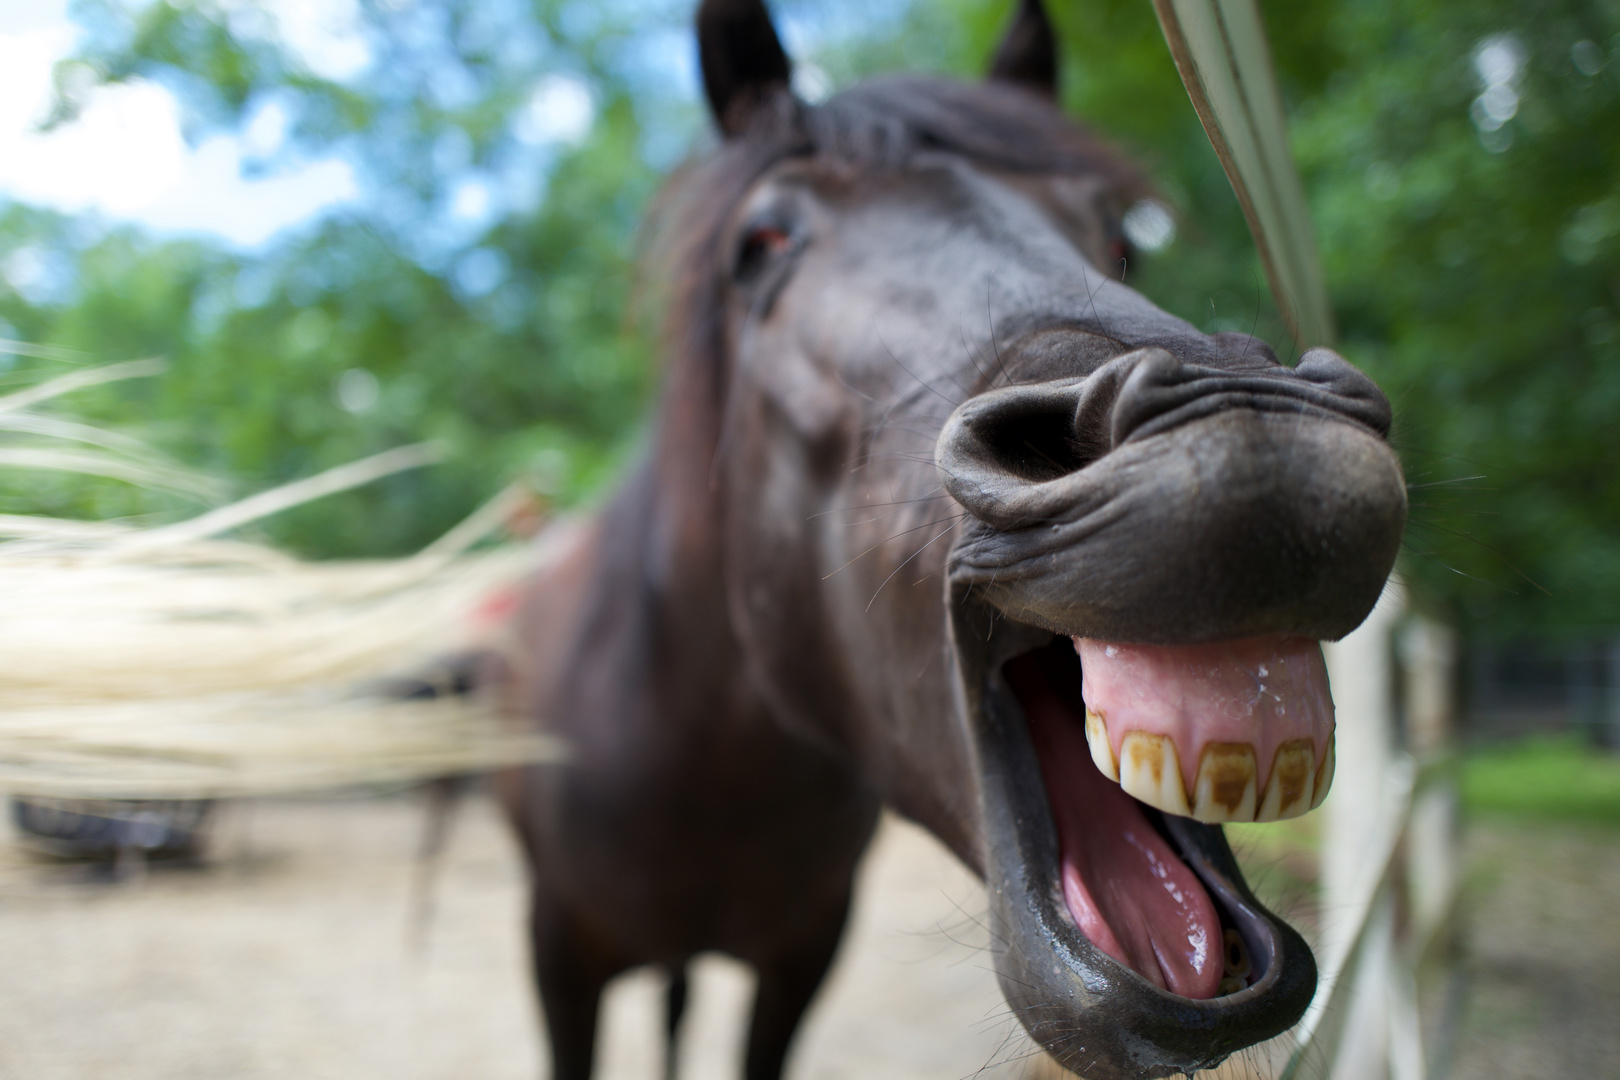
\includegraphics[width=0.7\textwidth]{Schaltskizze.jpg} % Schaltskizze einfügen
    \caption{Schaltskizze des Messaufbaus}
\end{figure}

\subsection{Messergebnisse}
Präsentiere die Messergebnisse, z.B. in Tabellenform oder grafisch. Vergleiche die Messergebnisse mit theoretisch erwarteten Werten und diskutiere etwaige Abweichungen.

\begin{table}[H]
    \centering
    \begin{tabular}{|c|c|c|}
        \hline
        Eingangsspannung & Gemessene Spannung & Abweichung \\
        \hline
        0.00 V & 0.00 V & -0.00 V \\
        0.00 V & 0.00 V & +0.00 V \\
        \hline
    \end{tabular}
    \caption{Messergebnisse des Versuchs}
\end{table}

\subsection{Diskussion}
Diskutiere die Messergebnisse. Was sind die wichtigsten Erkenntnisse? Was lief gut, was könnte verbessert werden?

\section{Versuch 2: DAC}

\subsection{Zielsetzung}
In diesem Versuch wurde die Funktionsweise eines Digital/Analog-Wandlers (DAC) untersucht, insbesondere seine Eigenschaften wie Monotonie, Linearität und Einschwingzeit. Ziel des Versuchs war es, die Monotonie und Linearität des DAC zu bestimmen sowie die Einschwingzeit bei einer Spannungsänderung zu messen. Diese Parameter sind entscheidend, um die Eignung des DAC für präzise analoge Anwendungen zu beurteilen.

\subsection{Bauteile und Messgeräte}
Verwendete Bauteile und Geräte:
\begin{itemize}
\item DAC ZN429E-8: DAC wandelt die digitalen Eingangssignale in analoge Spannungen um.
\item SN74LS74AN Flip-Flop: Triggerung und Kontrolle der Monotonie
\item Netzgerät: Bereitstellung der Versorgungsspannung
\item Fluke DMM: Messung der Versorgungs- und Ausgangsspannungen
\item Oszilloskop: Untersuchung der Signalformen und des Einschwingverhaltens
\end{itemize}

\subsection{Messkonzept}
Erkläre das Messkonzept und füge eine Schaltskizze ein, falls erforderlich. Beschreibe,
warum bestimmte Messmethoden oder Schaltungen verwendet wurden.

Der Versuchsaufbau basierte auf der Schaltung, die in der Versuchsanleitung beschrieben ist. Die Schaltskizze (siehe Anhang) zeigt den genauen Aufbau, bei dem der DAC und das Flip-Flop für die Monotonie- und Linearitätsmessungen verwendet wurden. Die Spannung wurde mithilfe des Oszilloskops kontinuierlich beobachtet, um mögliche Abweichungen der Ausgangsspannung bei Änderung des digitalen Eingangs zu dokumentieren. Für die Messung der Einschwingzeit wurde die Spannungssprungantwort des DAC analysiert.

\begin{figure}[H]
    \centering
    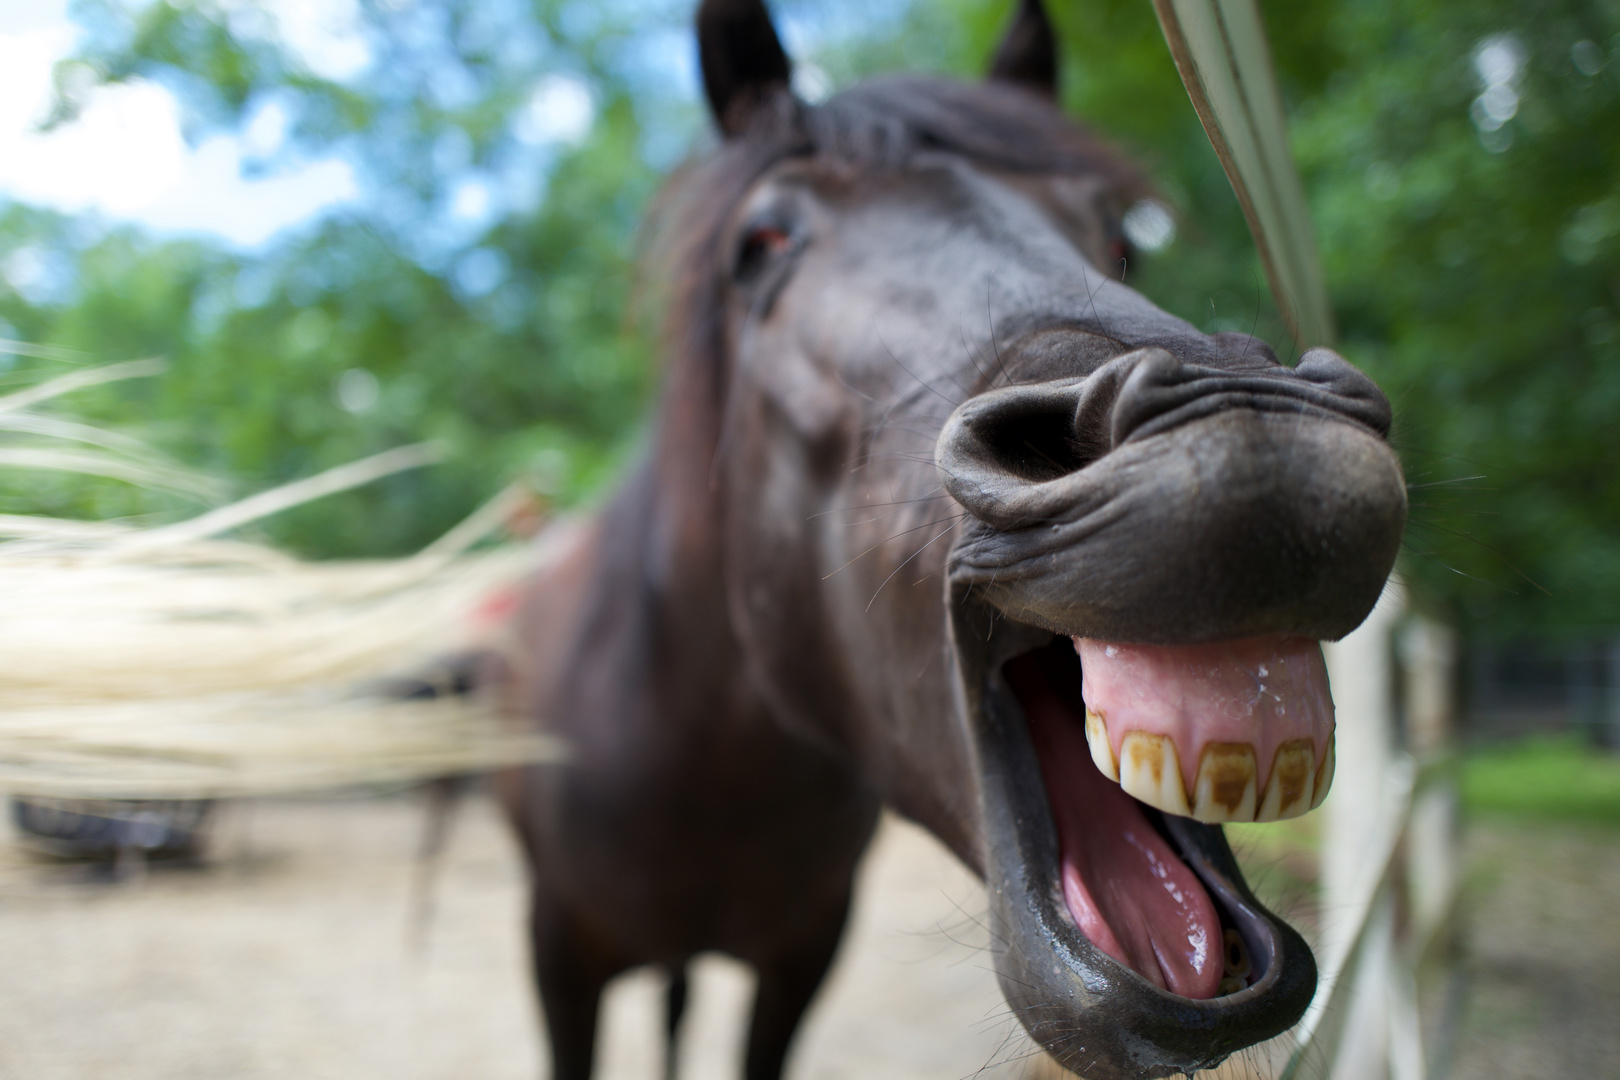
\includegraphics[width=0.7\textwidth]{Schaltskizze.jpg} % Schaltskizze einfügen
    \caption{Schaltskizze des Messaufbaus}
\end{figure}

\subsection{Messergebnisse}
Präsentiere die Messergebnisse, z.B. in Tabellenform oder grafisch. Vergleiche die Messergebnisse mit theoretisch erwarteten Werten und diskutiere etwaige Abweichungen.

Die Messergebnisse der Monotonie und Linearität wurden in Tabellenform und grafisch dargestellt. Aus diesen Werten ergaben sich kleinere Abweichungen vom idealen Verlauf, die jedoch im Rahmen der Spezifikationen des DAC liegen. Die detaillierten Ergebnisse können in der beiliegenden Excel-Datei gefunden werden.

\begin{table}[H]
    \centering
    \begin{tabular}{|c|c|c|}
        \hline
        Eingangsspannung & Gemessene Spannung & Abweichung \\
        \hline
        0.00 V & 0.00 V & -0.00 V \\
        0.00 V & 0.00 V & +0.00 V \\
        \hline
    \end{tabular}
    \caption{Messergebnisse des Versuchs}
\end{table}

\subsection{Diskussion}
Diskutiere die Messergebnisse. Was sind die wichtigsten Erkenntnisse? Was lief gut, was könnte verbessert werden?

\section{Fazit}
Ziehe ein Fazit über die Laborversuche. Was wurde gelernt? Welche Herausforderungen gab es?

\end{document}
